\chapter{Tutorial and Lab Allocation}

\section{Introduction}

After the lectures have been allocated, the next step is to allocate the tutorials. Since lectures occupy a major part of faculty bandwidth, they are allocated before tutorials, which can cover the remaining bandwidth of the faculty.

Tutorial and lab delivery have the materials and the structure already defined by the lecturer. Thus, less subject-matter expertise is required to deliver tutorials. This allows for more flexibility in the allocation of tutorials and makes more faculty members eligible to deliver tutorials out of their area of expertise.

However, this allocation needs to avoid fragmentation i.e. the tutorials of the same course should ideally be allocated to the same faculty. This is because the faculty would have to familiarise themselves with the course material of each course that they are allocated. Additionally, the students get a more consistent experience across all the components of the course if the same faculty delivers the lectures, tutorials, and labs of the same course.

To avoid fragmentation, batching of tutorials and labs is introduced, which involves grouping multiple sessions of a course tutorial into batches, and then allocating a batch of tutorials to the faculty, one batch at a time. This ensures that the same faculty gets the opportunity to teach multiple sessions of the same tutorial.  Additionally, the cost function is modified to bias the allocation of tutorials and labs to the same faculty who was allocated the lectures, tutorials, or labs of the same course. These two techniques, combined, result in the same faculty being preferably allocated the lectures, tutorials, and labs of a course.

Additional teaching duty limits are also introduced to ensure that faculty members receive a similar proportion of lectures, tutorials, and labs. It also helps avoid sparse workloads, where the faculty is allocated many small teaching duties, instead of a few large teaching duties, which results in additional workload overhead for the faculty.

An additional technique of dynamic limit relaxation is also introduced, which involves targeted relaxation of the workload limits of the faculty to accommodate the unallocated tutorials, avoiding widespread overload of the faculty to deal with the unallocated tutorials. All of the above steps are also applied to the lab allocation process.

In this chapter, a comprehensive approach to tutorial and lab allocation is discussed, which uses the Hungarian algorithm to allocate the tutorials and labs to faculty, while utilizing the techniques discussed above to meet the objectives and constraints of the tutorial and lab allocation problem. These techniques are then applied to a real-world dataset to evaluate their effectiveness.

\section{Defining the Tutorial Allocation Problem}

The tutorial allocation involves allocating tutorials to faculty members who are eligible to deliver them. Tutorial allocation is similar to lecture allocation, which means that the objectives and constraints of the tutorial allocation problem are similar to the lecture allocation problem. This means that the tutorial allocation problem is also a multi-objective optimization problem, with a set of objectives that need to be optimized and a set of constraints that need to be satisfied.

The objectives of the lecture allocation - ensure that all courses are allocated, ensure that the workload of faculty is distributed equitably, ensure that the proportion of lectures, tutorials, and labs allocated to each faculty is similar, ensure that earlier-year courses are allocated to the best faculty, to maximize the student feedback score and to maximize the faculty preferences - are also the objectives of the tutorial allocation problem.

However, there are a few additional considerations that need to be taken into account while modeling the tutorial allocation problem. These considerations are:

\begin{itemize}
  \item \textbf{Broader Availability of Faculty}

        Tutorials require less expertise in a particular subject area than lectures. Thus, tutorials can be delivered by a broader range of faculty. This allows for more flexibility in the allocation of tutorials. Thus, the tutorial allocation problem should be modeled in a way that the tutorials can be allocated to a broader range of faculty.

  \item \textbf{Preferring towards already allocated courses}

        The lectures, tutorials, and labs of the same course should ideally be allocated to the same faculty. This is because the faculty would have to familiarise themselves with the course material of each course that they are allocated. Additionally, having the same faculty deliver the lectures, tutorials, and labs of the same course would ensure that the students have a consistent experience across all the components of the course. Thus, the tutorial allocation problem should be modeled in a way that if the lectures of a course are allocated to a faculty, then they should get a higher preference for the tutorials of the same course.

  \item \textbf{Batching Tutorials}

        Tutorials are smaller pieces of work that are more numerous than lectures. Thus, it is not feasible to allocate tutorials one at a time, since it would lead to too many iterations. Additionally, allocating tutorials one at a time may lead to every tutorial session being allocated to a different faculty, which would lead to a lot of faculty having to familiarise themselves with the course material of a lot of courses, and the students. Thus, the tutorial allocation problem should be modeled in a way that the tutorials are allocated in batches.

\end{itemize}

As a result, the tutorial allocation problem is modeled differently from the lecture allocation problem. The next section discusses how the tutorial allocation problem is modeled.

\section{Modelling the Tutorial Allocation Problem}

The tutorial allocation problems, similar to the lecture allocation problem, can be modeled as an assignment problem where the tasks are the tutorials, and the resources are the faculty. Every tutorial will be assigned to exactly one faculty, but multiple tutorials or labs can be assigned to the same faculty, i.e. the tutorial allocation problems are many-to-one assignment problems.

The cost of allocating a tutorial to a faculty should take into consideration the student feedback and the faculty preferences. Additionally, the cost should be modeled such that consistency of courses can be maintained for tutorials.

The allocation process should also handle the management priority of allocating earlier-year courses to the best faculty. Additionally, the allocation process should ensure that the workload of faculty is distributed equitably and that a similar proportion of lectures, tutorials, and labs are allocated to each faculty.

\subsection{Allocating using the Hungarian Algorithm}

Similar to the lecture assignment problem, the tutorial assignment is performed using the Hungarian algorithm. Since the algorithm only works for one-to-one assignment problems, the tutorial assignment problem is converted into a one-to-one assignment problem by running multiple iterations of the algorithm, where each iteration allocates exactly one session of tutorials to the faculty.

The cost function for the lecture allocation problem is used as a starting point to define the cost function for the tutorial allocation problem. Thus, \autoref{eq:course_faculty_fit} is used as the course-faculty fit metric for the problem. This fit metric is then used to construct the allocation matrix as defined in \autoref{alg:cost_matrix_construction}. This cost matrix function is then used as input to the Hungarian algorithm, similar to the lecture allocation problem defined in \autoref{alg:base_lec_alloc}.

For the cost function, a separate set of student feedback and faculty preferences are provided for tutorials, to account for the different faculty delivering the tutorials, and the different student experience in tutorials. The faculty preferences for tutorials also tend to be broader, with more faculty being able to deliver tutorials than lectures.

However, the allocation process has a key difference - the tutorials involve multiple sessions of the same tutorial, each of which may be allocated to the same faculty as well. However since Hungarian only allocates one task to one agent at a time, if multiple sessions of one tutorial are allocated in a single iteration, they will never be allocated to the same faculty. This would lead to the tutorials of the same course being allocated to different faculty, which leads to problems discussed previously.

As a result, the tutorial allocation process is modified to allocate only one session of each tutorial in each iteration. This ensures that the same faculty gets the opportunity to teach multiple sessions of the same tutorial. The allocation algorithm is thus defined as shown below.

\begin{algorithm}[H]
  \caption*{Base Tutorial Allocation Algorithm}
  \begin{algorithmic}
    \Procedure{AllocateTutorials}{$tutorials, faculty$}
    \State $unallocatedTutorialSessions \gets tutorials$
    \State $allAllocations \gets \emptyset$
    \While{$unallocatedTutorialSessions \neq \emptyset$}
    \State $iterationSessions \gets getFirstUnallocatedSession()$
    \State $costMatrix \gets constructCostMatrix(iterationSessions, faculty)$
    \State $allocation \gets \text{HungarianAlgorithm}(costMatrix)$
    \State $allAllocations \gets allAllocations \cup allocation$
    \State $unallocatedTutorialSessions \gets unallocatedTutorialSessions \setminus allocation$
    \EndWhile
    \State \textbf{return} $allAllocations$
    \EndProcedure
  \end{algorithmic}
\end{algorithm}

where, $tutorials$ is the set of all tutorials, and $faculty$ is the set of all faculty. The $constructCostMatrix$ function is defined as shown in \autoref{alg:cost_matrix_construction}. In every iteration, the allocation process takes the first unallocated tutorial session of each course and allocates it to a faculty. This ensures that the same faculty gets the opportunity to teach multiple sessions of the same tutorial.

In the next section, the cost function is modified to improve the consistency of courses, prioritize earlier-year courses, and ensure equitable distribution of workload.

\section{Designing the Cost Function}

As mentioned in the previous section, the course-faculty fit metric is used and defined in the lecture allocation process as the starting point for the cost function for the tutorial allocation problem. This fit metric is then used to construct the allocation matrix as defined in \autoref{alg:cost_matrix_construction}, which serves as the input to the Hungarian algorithm. However, the cost function needs to be modified to account for the different objectives and constraints of the tutorial allocation problem.

Firstly, to maintain the consistency of courses, the cost function is modified to bias the allocation of tutorials to the same faculty who was allocated the lectures, tutorials, or labs of the same course. This is done by reducing the cost of allocating a tutorial to the faculty by a certain bias if the faculty was allocated any existing tutorials or labs of the same course. Additionally, even if the faculty was allocated the lectures of the same course, the cost of allocating a tutorial to the faculty is reduced by the same bias, since the lectures, tutorials, and labs of the same course should ideally be allocated to the same faculty.

Since the tutorial allocation process does not iterate over the tutorial sessions year-wise to achieve the management priority, the cost function is modified to bias the allocation of earlier-year courses to the best faculty. This is done by reducing the cost of allocating a tutorial to a high-quality faculty and increasing the cost of allocating a tutorial to a low-quality faculty, to ensure that the better faculty are allocated the earlier-year courses. This bias is defined separately for each year, to allow for different degrees of prioritization for different year courses, with the bias being higher for earlier-year courses.

Finally, the cost function is modified to ensure that the workload of faculty is distributed equitably. This is done by limiting the total number of teaching duties that can be allocated to each faculty, as well as a limit to each of the lectures, tutorials, and labs that can be allocated to each faculty. If the faculty has exceeded the workload limit, then the cost of allocating a tutorial to the faculty is set to infinity. This ensures that the faculty isn't overloaded with a sparse and fragmented workload.

\subsection{Preferring Already Allocated Courses}

The allocation process runs multiple iterations of the Hungarian algorithm, each iteration allocating one session of tutorials to faculty, which ensures that the same faculty gets the opportunity to teach multiple tutorial sessions of the same course. Although the multiple iterations of the algorithm allow for the same faculty to be allocated to multiple sessions of tutorials, there is no mechanism in the process to prefer the same faculty across multiple iterations of the algorithm.

The algorithm needs to be modified with a mechanism to prefer a faculty for a tutorial if the same faculty was allocated to previous sessions of tutorials for the same course. Additionally, the algorithm needs to prefer a faculty for the tutorials of a course if the same faculty was allocated the lectures of the same course. This would ensure a consistent experience for the students across all the components of the course.

To do this, the cost function has to be modified to bias the allocation of tutorials to the same faculty who was allocated the lectures, tutorials, or labs of the same course. This is done by reducing the cost of allocating a tutorial to the faculty by a certain bias if the faculty was allocated the lectures, tutorials, or labs of the same course. This bias is configurable and can be adjusted based on the management's preference towards consistency of courses. For the test dataset, a bias of 1 was found to be optimal, but this is a configurable parameter that can be adjusted based on the requirements of the institution.

With the bias, the modified cost matrix function is defined as shown below. The parameter $consistencyBias$ is configurable and can be adjusted based on the management's preference towards consistency of courses. For the test dataset, a bias of 1 was found to be optimal, but this is a configurable parameter that can be adjusted based on the requirements of the institution.

\begin{algorithm}[H]
  \caption*{Refinement 1: Incorporating Consistency Bias}
  \begin{algorithmic}
    \Procedure{ConstructCostMatrix}{$tutorials, faculty, existingAllocations$}
    \State $costMatrix \gets \emptyset$
    \For{$tutorial \in tutorials$}
    \For{$f \in faculty$}
    \State $costMatrix[tutorial][f] \gets \Call{Q}{tutorial, f}$
    \If{$f \in existingAllocations[tutorial.course]$}
    \State $costMatrix[tutorial][f] \gets costMatrix[tutorial][f] - consistencyBias$
    \EndIf
    \EndFor
    \EndFor
    \State \textbf{return} $costMatrix$
    \EndProcedure
  \end{algorithmic}
\end{algorithm}

where $existingAllocations$ is the set of all lectures, tutorials, and labs that have already been allocated.

\subsection{Handling Management Priority}

In the lecture allocation problem, the management priority of allocating earlier-year courses to the best faculty was handled by allocating the courses year-wise. This was done by allocating the courses of the first year first, then the courses of the second year, and so on. However, this approach is not feasible for the tutorial allocation problem, since ensuring consistency of courses already requires multiple iterations of the algorithm. Allocating the courses year-wise would lead to too many iterations of the algorithm, and would also lead to local optima, where the algorithm allocates too many tutorials to the same faculty for earlier-year courses, and then is unable to allocate the tutorials of later-year courses to the same faculty.

Additionally, since the tutorial sessions are secondary teaching duties, providing a supplementary experience to the lectures, it is not as important to reserve the best faculty for the earlier-year courses. The tutorial sessions also don't require as much expertise in the particular subject area as the lectures and thus aren't affected as much by the quality of the faculty. Thus, the allocation process is modified to allocate the tutorials of all years at once, instead of allocating the tutorials year-wise.

However, the management priority of allocating earlier-year courses to the best faculty still needs to be handled. This is done by skewing the cost function to prioritize better faculty for earlier years. For earlier-year courses, the cost of allocating a high-quality faculty is reduced, and the cost of allocating a low-quality faculty is increased, to ensure that the better faculty are allocated the earlier-year courses. To achieve this, a bias factor is introduced, which is added or subtracted from the cost of allocating a faculty to a tutorial. This bias factor is configurable and can be adjusted based on the management's preference towards allocating earlier-year courses to the best faculty. The bias also has a different value for each year, to allow for different degrees of prioritization for different year courses.

To differentiate high-quality faculty from low-quality faculty, a quality threshold is defined. If the cost of allocating a faculty to a tutorial is less than the quality threshold, then the faculty is considered to be high quality and the bias is subtracted from the cost. If the cost of allocating a faculty to a tutorial is greater than the quality threshold, then the faculty is considered to be low quality and the bias is added to the cost.

\begin{table}[H]
  \centering
  \begin{tabular}{|c|c|c|c|c|c|}
    \hline
    Year & 1 & 2    & 3   & 4    & 5 \\ \hline
    Bias & 1 & 0.75 & 0.5 & 0.25 & 0 \\ \hline
  \end{tabular}
  \caption{Year-wise Bias for Tutorial Allocation}
  \label{tab:yearwise_bias}
\end{table}

With the bias, the modified cost matrix function is defined as shown below. The $qualityThreshold$ and $yearwiseBias$ parameters are configurable and can be adjusted based on the management's preference towards allocating earlier-year courses to the best faculty. For the test dataset, the biases are defined in \autoref{tab:yearwise_bias}. The $qualityThreshold$ is defined as 1, which means that any faculty with a cost of 1 or less is considered to be high quality, and any faculty with a cost of 1 to 5 is considered to be low quality.


\begin{algorithm}[H]
  \caption*{Refinement 2: Incorporating Year-wise and Consistency Bias}
  \begin{algorithmic}
    \Procedure{ConstructCostMatrix}{$tutorials, faculty, existingAllocations$}
    \State $costMatrix \gets \emptyset$
    \For{$tutorial \in tutorials$}
    \For{$f \in faculty$}
    \State $cost \gets \Call{Q}{tutorial, f}$
    \State $year = tutorial.course.year$
    \If{$cost \leq qualityThreshold$}
    \State $cost \gets cost - yearwiseBias[year]$
    \Else
    \State $cost \gets cost + yearwiseBias[year]$
    \EndIf
    \If{$f \in existingAllocations[tutorial.course]$}
    \State $cost \gets cost - consistencyBias$
    \State $costMatrix[tutorial][f] \gets cost$
    \EndIf
    \EndFor
    \EndFor
    \State \textbf{return} $costMatrix$
    \EndProcedure
  \end{algorithmic}
\end{algorithm}

where $existingAllocations$ is the set of all lectures, tutorials, and labs that have already been allocated.

\subsection{Distributing Teaching Duties Equitably}
\label{sec:workload_limits}

The tutorial allocation process should ensure that the teaching duties are distributed equitably amongst faculty. One part of this is ensuring that a similar proportion of lectures, tutorials, and labs are allocated to each faculty. This means that if the institution has a certain proportion of lectures, tutorials, and labs, then the allocation of each faculty should ideally have a similar proportion of lectures, tutorials, and labs. To achieve this, a mechanism needs to be introduced to limit the workload of lectures, tutorials, and labs that can be allocated to each faculty.

Thus, the workload limits of the faculty are introduced with the same proportion of lectures, tutorials, and labs as the institution. This is done incrementally, by first setting the workload limits of the faculty to only the proportion of lectures, then increasing the workload limits to include the proportion of tutorials, and then increasing the workload limits to include the proportion of labs. This ensures that the workload of the faculty mimics the workload of the institution, and thus a similar proportion of lectures, tutorials, and labs are allocated to each faculty.

For example, if the institute's workload consists of 60\% lectures, 20\% tutorials, and 20\% labs, then during the lecture allocation process the workload limits of the faculty are set to only 60\% of the total workload limit of the faculty. This ensures that the lecture allocation process allocates only 60\% of the total workload limit of the faculty to lectures. Then for the tutorial allocation process, the workload limits are increased to 80\% of the total workload limit of the faculty. And then finally, for the lab allocation process, the workload limits are increased to 100\% of the total workload limit of the faculty.

This also means that if a faculty was under-allocated lectures, which can happen to result from various factors like their preferences or student feedback, then the faculty would be allocated more tutorials to compensate for the under-allocation of lectures. This ensures that, while the workload of the faculty is distributed in a similar proportion to the workload of the institution, the faculty workload isn't underutilized.

The second part of the workload distribution is ensuring that the workload of the faculty isn't too fragmented. This means that the faculty shouldn't be overloaded with many small teaching duties, which might be able to fit within the workload limits of the faculty, but would lead to a lot of overhead for the faculty in terms of preparation and delivery, as well as commuting between the different teaching duties. To achieve this, a limit is put on the total number of teaching duties that can be allocated to each faculty Additionally, a limit to each of the lectures, tutorials, and labs is also added.

These teaching duty limits are defined separately for professors and lecturers, since lecturers are expected to have fewer research commitments than professors, and can thus be allocated more teaching duties. The limits used in the test dataset are defined in \autoref{tab:teaching_duty_limits}.

\begin{table}[H]
  \centering
  \begin{tabular}{|c|c|c|c|c|}
    \hline
    Faculty Type & Total & Lectures & Tutorials & Labs \\ \hline
    Professor    & 10    & 3        & 5         & 6    \\ \hline
    Lecturer     & 20    & 3        & 10        & 12   \\ \hline
  \end{tabular}
  \caption{Teaching Duty Limits for Faculty}
  \label{tab:teaching_duty_limits}
\end{table}

The final cost matrix function is defined as a procedure in \autoref{alg:tutorial_allocation}.

\section{Batch Allocation of Tutorials}

Another way to improve the consistency of courses is to allocate the tutorials in batches. This involves dividing the tutorials into batches of multiple tutorials and then allocating one batch of tutorials at a time to the faculty. This ensures that the faculty is assigned at least a few sessions of the same tutorial, which improves the consistency of courses. This adds a certainty that the algorithm will allocate the faculty densely, allocating more sessions of the same tutorial to the same faculty in order to ensure consistency of courses.

Additionally, since the tutorial allocation problem is completed in multiple iterations, each iteration of the algorithm assigning one tutorial to one faculty, the allocation process can take a long time to complete. This is because one course can have a large number of students studying the course. For this, a large number of tutorials need to be allocated, since each tutorial session can only accommodate a limited number of students. For a course with 800 students, 26 separate tutorial sessions are needed, each with around 30 students. This means that at least 26 separate iterations of the algorithm need to be run to allocate all the tutorials for the course.

To achieve this, the tutorial allocation algorithm is modified to allocate the tutorials in batches. This is done by creating a batch of tutorials, and then allocating the batch to faculty. This ensures that the algorithm allocates the tutorials densely, allocating more sessions of the same tutorial to the same faculty. This also reduces the number of iterations of the algorithm that need to be run, since the algorithm allocates multiple tutorials in one iteration.

Determining the correct batch size is important since a batch size that is too large would require higher workload limits to accommodate the entire batch of tutorials, leading to unallocated tutorials and sub-optimal faculty utilization. However, a batch size that is too granular would lead to fragmentation of the course tutorials, with multiple faculty being allocated to the tutorials of the same course. Additionally, smaller batch sizes also result in a slower allocation process due to more iterations required.

The batch size is a configurable parameter that can be adjusted based on the requirements of the institution. It is a function of the management's preference towards consistency, as well as the availability of faculty to deliver the tutorials. For tutorials, a batch size of 6 was found to be optimal for the test dataset, to provide optimal granularity while ensuring consistency of courses.

With the batch allocation, the tutorials are divided into batches of size $batchSize$ before the allocation begins, and then the algorithm is modified to select the first unallocated batch of tutorials for cost matrix construction, instead of the first unallocated session.


\section{Dynamically Adjusting Workload Limits for Feasibility}

Although the tutorial allocation process manages to allocate most of the tutorials, some tutorials may remain unallocated. This may be due to the workload limits of the faculty, which may not be able to accommodate all the tutorials. It may also be due to the teaching duty limits of the faculty, which limit the number of tutorials and the total number of teaching duties that can be allocated to the faculty.

However, allocation of all the tutorials is the primary objective of the tutorial allocation process. Thus, additional measures need to be added to the allocation process to ensure that all the tutorials are allocated to faculty, even at the cost of exceeding the workload limits or the teaching duty limits of the faculty.

To achieve this, a method of dynamically adjusting the workload limits of the faculty is introduced. This involves identifying the cause of the infeasibility, i.e. whether the workload limit of the faculty or the teaching duty limits that can be allocated to each faculty is responsible for the infeasibility. Then the workload limits of the faculty or the teaching duty limits are adjusted respectively, to accommodate the unallocated tutorials.

This process is repeated, iteratively rectifying the cause of the infeasibility, until all the tutorials are allocated to faculty. This ensures that the tutorial allocation process is able to allocate all the tutorials to faculty, even if it means exceeding the workload limits or the teaching duty limits of the faculty.

To find the cause of infeasibility, the process looks at the unallocated tutorials. For each unallocated tutorial, then it checks if there are existing faculty who have been allocated to other tutorials of the same course. For these faculty, it checks if they have exceeded their workload limits, if yes then it increases their workload limits to accommodate the unallocated tutorials. It also checks if their teaching duty limits have been exceeded, if yes then it increases their teaching duty limits to accommodate the unallocated tutorials. In the absence of already allocated faculty, it looks for the faculty with the lowest workload utilization and repeats the same process for them. This process is repeated until all the tutorials are allocated to faculty or a predefined maximum for the workload limit is reached.

For each iteration, the workload limit of the faculty is increased by 10\% of the total workload limit of the faculty.

\begin{algorithm}[H]
  \caption*{Dynamic Limit Relaxation Algorithm}
  \begin{algorithmic}
    \Procedure{RelaxWorkloadLimits}{}
    \While {$unallocatedTutorials \neq \emptyset$}
    \For {$tutorial \in unallocatedTutorials$}
    \State $alreadyAllocatedFaculty \gets existingAllocations[tutorial.course]$
    \If{$alreadyAllocatedFaculty \neq \emptyset$}
    \For{$f \in alreadyAllocatedFaculty$}
    \State $wLimit, tLimit \gets \Call{CheckLimits}{f}$
    \EndFor
    \Else
    \State $f \gets \text{Faculty eligible to teach $tutorial$ with lowest workload}$
    \State $wLimit, tLimit \gets \Call{CheckLimits}{f}$
    \EndIf
    \EndFor
    \If{$wLimit and workloadLimit \leq maxWorkloadLimit$}
    \State $workloadLimit \gets workloadLimit + 0.1$
    \EndIf
    \If{$tLimit$}
    \State $totalTeachingDutyLimit \gets totalTeachingDutyLimit + 1$
    \State $tutorialLimit \gets tutorialLimit + 1$
    \EndIf
    \State Attempt to allocate tutorials again
    \EndWhile
    \EndProcedure
    \\
    \Procedure{CheckLimits}{$faculty$}
    \State $expandWorkloadLimit = \text{False}$
    \State $expandTeachingDutyLimit = \text{False}$
    \If{$faculty$ has exceeded \textbf{total teaching duty limit} or \textbf{tutorial limit}}
    \State $expandTeachingDutyLimit \gets \text{True}$
    \EndIf
    \If{$faculty.workload \geq faculty.workloadLimit$}
    \State $expandWorkloadLimit \gets \text{True}$
    \EndIf
    \State \Return $expandWorkloadLimit, expandTeachingDutyLimit$
    \EndProcedure
  \end{algorithmic}
\end{algorithm}

where $unallocatedTutorials$ is the set of all unallocated tutorials, $existingAllocations$ is the set of all lectures, tutorials, and labs that have already been allocated, and $faculty$ is the set of all faculty. The $maxWorkloadLimit$ is the maximum workload limit that can be allocated to a faculty and is defined as 1.5 times the total workload limit of the faculty.

\section{The Tutorial Allocation Process}

In the tutorial allocation algorithm, the tutorial sessions are divided into batches of size of $batchSize$. Then, the algorithm runs multiple iterations of the Hungarian algorithm, each iteration allocating one batch of tutorials to the faculty. In each iteration, the algorithm constructs the cost matrix using the cost matrix function defined below, which takes into account the consistency of courses, the management priority of allocating earlier-year courses to the best faculty, and ensures the workload limits of the faculty are not exceeded. The algorithm then allocates the tutorials to faculty and then repeats the process until all the batches of tutorials have been allocated. This algorithm is defined in \autoref{alg:tutorial_allocation}.

\begin{algorithm}[H]
  \caption{Tutorial Allocation Algorithm}
  \begin{algorithmic}
    \Procedure{AllocateTutorials}{$tutorials, faculty$}
    \State $allAllocations \gets \emptyset$
    \State $unallocatedBatches \gets divideIntoBatches(tutorials, batchSize)$
    \While{$unallocatedBatches \neq \emptyset$}
    \State $iterationBatches \gets \text{First Unallocated Batch per Course}$
    \State $costMatrix \gets \Call{ConstructCostMatrix}{iterationBatches}$
    \State $allocation \gets \text{HungarianAlgorithm}(costMatrix)$
    \State $allAllocations \gets allAllocations \cup allocation$
    \State $unallocatedBatches \gets unallocatedBatches \setminus allocation$
    \EndWhile
    \State \textbf{return} $allAllocations$
    \EndProcedure
    \\
    \Procedure{ConstructCostMatrix}{$batches$}
    \State $costMatrix \gets \emptyset$
    \For{$batch \in batches$}
    \For{$f \in faculty$}
    \State $cost \gets \Call{Q}{batch, f}$
    \State $year = batch.course.year$
    \If{$cost \leq qualityThreshold$}
    \State $cost \gets cost - yearwiseBias[year]$
    \Else
    \State $cost \gets cost + yearwiseBias[year]$
    \EndIf
    \If{$f \in existingAllocations[batch.course]$}
    \State $cost \gets cost - consistencyBias$
    \EndIf
    \If {$f$ has exceeded \textbf{total teaching duty limit} or \textbf{tutorial limit}}
    \State $cost \gets \infty$
    \EndIf
    \State $costMatrix[batch][f] \gets cost$
    \EndFor
    \EndFor
    \State \textbf{return} $costMatrix$
    \EndProcedure
  \end{algorithmic}
  \label{alg:tutorial_allocation}
\end{algorithm}

where, $tutorials$ is the set of all tutorials, $faculty$ is the set of all faculty, and $batchSize$ is the size of the batch of tutorials. The $divideIntoBatches$ function just divides the tutorials into batches of size $batchSize$. If the number of tutorials is not a multiple of $batchSize$, then the last batch will have less than $batchSize$ tutorials.

The $constructCostMatrix$ function is defined in the second procedure, which incorporates the teaching duty limits, the year-wise bias, the consistency bias, and the workload limits of the faculty. The $qualityThreshold$, $consistencyBias$, $yearwiseBias$, and workload limits for every faculty are defined in the previous chapters. Each of these parameters is configurable and can be adjusted as per the needs of the institution. The $existingAllocations$ is the set of all lectures, tutorials, and labs that have already been allocated.

Additionally, the pre-allocation step, from the lecture allocation process, is also incorporated. Pre-Allocation involves identifying the tutorial batches which have a shortage of faculty, and allocating them to faculty before the main allocation process begins. This is done because the main allocation process isn't aware of faculty shortages, and thus might allocate the faculty needed for such courses to other faculty to optimize the cost function, which would lead to unallocated tutorials.

The dynamic limit relaxation process replaces the workload relaxation process from the lecture allocation process and is thus not applied

The post-allocation step was not found to be useful, since it primarily helped with unallocated lectures caused by the management priority of allocating earlier-year courses to the best faculty. Since the tutorial allocation process doesn't allocate the tutorials year-wise, and instead uses the year-wise bias to allocate earlier-year courses to the best faculty, the post-allocation step was found to be unhelpful.

The entire allocation flow used is defined as shown in \autoref{fig:tutorial_allocation_flow}.

\begin{figure}[H]
  \centering
  \begin{tikzpicture}[node distance=0.5cm]
    \node (start) [startstop] {Start};
    \node (workload_limits) [process, below=of start] {Increase Workload Limits};
    \node (batch) [process, below=of workload_limits] {Divide into Batches};
    \node (preallocation) [process, below=of batch] {Pre-Allocation};
    \node (iter) [process, below=of preallocation] {Allocate Tutorial Batches};
    \node (workload_check) [decision, below=of iter] {All Allocated?};
    \node (workload) [process, right=of workload_check, xshift=0.25cm] {Dynamically Adjust Limits};
    \node (stop) [startstop, below=of workload_check, yshift=-0.25cm] {Stop};

    \draw [arrow] (start) edge (workload_limits)
    (workload_limits) edge (batch)
    (batch) edge (preallocation)
    (preallocation) edge (iter)
    (iter) edge (workload_check)
    (workload_check) edge node[anchor=south] {No} (workload)
    (workload_check) edge node[anchor=east] {Yes} (stop)
    (workload) edge[out=270, in=90] (stop);
    \node [draw=red, fit=(workload_limits) (batch), inner sep=0.25cm, dashed, label={left:Preparation}] {};
    \node [draw=red, fit=(preallocation) (iter), inner sep=0.25cm, dashed, label={left:Allocation}] {};
    \node [draw=red, fit=(workload_check) (workload), inner sep=0.25cm, dashed, label={left:Fixing Unallocated Tutorials}] {};
  \end{tikzpicture}
  \caption{Tutorial Allocation Flow}
  \label{fig:tutorial_allocation_flow}
\end{figure}

The process begins by increasing the workload limits of the faculty to include tutorials. Then, the tutorial sessions are divided into batches of size $batchSize$. Then the pre-allocation process is run, which allocates the tutorials that have a shortage of faculty. Then, the algorithm runs multiple iterations of the allocation, each iteration allocating one batch of tutorials to the faculty. In each iteration, the algorithm constructs the cost matrix which takes into account the consistency of courses, the management priority of allocating earlier-year courses to the best faculty, and ensures the workload limits of the faculty are not exceeded. The Hungarian algorithm then allocates the tutorials to faculty and then repeats the process until all the batches of tutorials have been allocated. This is followed by dynamically adjusting the workload limits and teaching duty limits of the faculty to accommodate the tutorials that have not been allocated, if the need arises.

\section{The Lab Allocation Process}

The lab allocation process is identical to the tutorial allocation process and is carried out right after the tutorial allocation process. For this, the workload limits are expanded to include labs as described in \autoref{sec:workload_limits}. Then the labs are pre-allocated, during which allocates the labs that have a shortage of faculty. Then multiple iterations of the allocation are run, each iteration allocating one batch of labs to faculty. In each iteration, the algorithm constructs the cost matrix, which is then used by the Hungarian algorithm to allocate the labs to faculty. This is followed by dynamic limit relaxation, which relaxes the workload limits and teaching duty limits of the faculty to accommodate the labs that have not been allocated.

The lab allocation uses the same cost matrix construction function as the tutorial allocation process, which involves the year-wise bias, the consistency bias, and the workload limits of the faculty. The same $qualityThreshold$, $consistencyBias$, and $yearwiseBias$ as the tutorial allocation process are used. The lab duty limit for professors is set to 6, and that for lecturers is set to 12. This is because the workload of labs is considered to be lower than the workload of tutorials, and thus more sessions can be allocated to faculty. These teaching duty limits are defined in \autoref{tab:teaching_duty_limits}.

The lab allocation process also uses batching of labs to improve the consistency of courses. The optimal batch size for labs was also found to be 6, which is odd since labs are typically twice as long as tutorials. However, because the workload per hour of the lab is considered to be lower than the workload per hour of tutorial, the two factors balance out, and the optimal batch size for labs is also 6. This also makes intuitive sense since workload granularity is of primary importance, not the number of hours allocated to each faculty.


\section{Experimental Results}

The tutorial allocation process uses the Hungarian algorithm to allocate the tutorials to faculty in batches. The algorithm is run multiple times, each time allocating one batch of tutorials to faculty. The algorithm is run until as many tutorials as possible are allocated to faculty, and then the unallocated tutorials are resolved by expanding the workload limits of the faculty, and if that fails, by reshuffling the allocations of the tutorials through the post-allocation process.

Using this approach, the tutorial allocation algorithms were run on the dataset of the School of Computer Science and Engineering, Nanyang Technological University, Singapore. The results of this allocation are shown below.

\begin{table}[ht]
  \centering
  \begin{tabular}{|l|c|c|}
    \hline
    \textbf{Metric} & \textbf{Tutorial} & \textbf{Lab} \\ \hline
    Assigned        & 522               & 491          \\
    Assigned Hrs    & 6758              & 5076         \\ \hline
    Unassigned      & 0                 & 0            \\
    Unassigned Hrs  & 0                 & 0            \\ \hline
    Avg Score       & 3.59              & 3.48         \\
    \hline
  \end{tabular}
  \caption{Tutorial Allocation Results}
  \label{tab:tut_lab_allocation_results}
\end{table}

\autoref{tab:tut_lab_allocation_results} shows the results of the tutorial allocation process. The process was able to allocate 522 out of 522 tutorials, and 491 out of 491 labs. In hours, this is 6758 out of 6758 tutorial hours, which is 100\% of the total tutorial hours, and 5076 out of 5076 lab hours, which is 100\% of the total lab hours.

\begin{figure}[H]
  \centering
  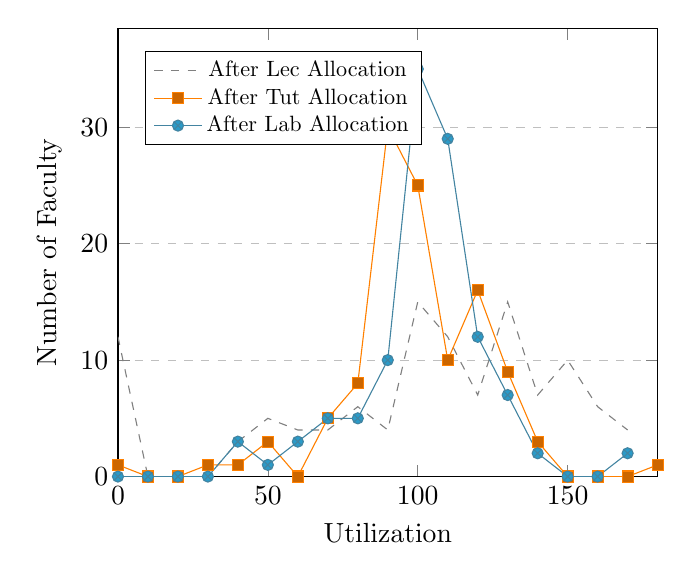
\begin{tikzpicture}
    \begin{axis}[
        xlabel={Utilization},
        ylabel={Number of Faculty},
        xmin=0, xmax=180,
        ymin=0,
        ymajorgrids=true,
        grid style=dashed,
        cycle list name=exotic,
        legend style={at={(0.05,0.95)}, anchor=north west, nodes={scale=0.80, transform shape}}
      ]
      \addplot[color=gray, dashed]
      coordinates {
          (0, 12) (10, 0) (20, 0) (30, 0) (40, 3) (50, 5) (60, 4) (70, 4) (80, 6) (90, 4) (100, 15) (110, 12) (120, 7) (130, 15) (140, 7) (150, 10) (160, 6) (170, 4)
        };
      \addlegendentry{After Lec Allocation}
      \addplot
      coordinates {
          (0, 1) (10, 0) (20, 0) (30, 1) (40, 1) (50, 3) (60, 0) (70, 5) (80, 8) (90, 30) (100, 25) (110, 10) (120, 16) (130, 9) (140, 3) (150, 0) (160, 0) (170, 0) (180, 1) (200, 1)
        };
      \addlegendentry{After Tut Allocation}
      \addplot
      coordinates {
          (0, 0) (10, 0) (20, 0) (30, 0) (40, 3) (50, 1) (60, 3) (70, 5) (80, 5) (90, 10) (100, 35) (110, 29) (120, 12) (130, 7) (140, 2) (150, 0) (160, 0) (170, 2)
        };
      \addlegendentry{After Lab Allocation}
    \end{axis}
  \end{tikzpicture}
  \caption{Faculty Utilization for Tutorial Allocation}
  \label{fig:tut_faculty_utilization}
\end{figure}

\autoref{fig:tut_faculty_utilization} shows the utilization of faculty for the tutorial allocation process. The utilization of faculty is defined as the number of hours allocated to the faculty divided by the total workload limit of the faculty. This also means that the utilization of faculty is inclusive of the lecture allocation process since the lecture allocation process is run before the tutorial allocation process.

One consistent pattern that can be seen in the utilization of faculty is that optimal utilization of faculty, i.e. 100\% utilization, is achieved for more faculty as the tutorial allocation processes are completed, while over-utilized and under-utilized faculty remain nearly constant. This is because many more faculty are available to teach tutorials than lectures, as previously discussed, the broader availability resulting from the lower expertise required to teach tutorials. It can be seen that the number of faculty with 0\% utilization decreases from 12 to 0, which confirms the above finding.

Relatively few faculty are over-utilized, with only 11 faculty having a utilization of more than 120\%. This is because the overutilization of faculty in lecture allocation was the overutilization of lecture workload limits. However, since the workload limits of the faculty are increased to include tutorials, the originally over-utilized faculty are no longer over-utilized.

\subsection{Impact of Consistency Bias}

The consistency bias is a configurable parameter that can be adjusted based on the requirements of the institution. To measure the impact of the consistency bias, the tutorial allocation process was run on the test dataset with different values of the consistency bias. The batching of tutorials was disabled for this test, to ensure that the impact of the consistency bias is isolated.

\begin{figure}[H]
  \begin{subfigure}[ht]{0.5\linewidth}
    \centering
    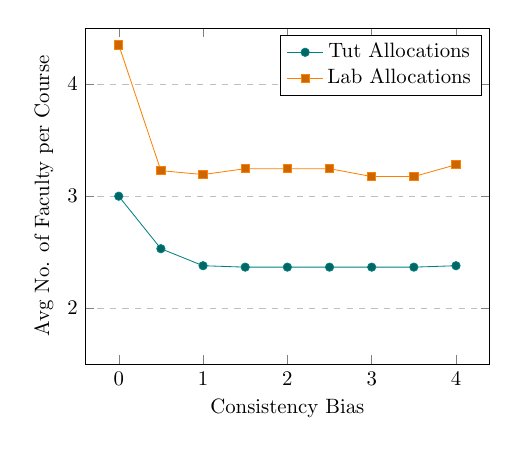
\begin{tikzpicture}[xscale=0.75, yscale=0.75]
      \begin{axis}[
          xlabel={Consistency Bias},
          ylabel={Avg No. of Faculty per Course},
          ymin=1.5, ymax=4.5,
          ymajorgrids=true,
          grid style=dashed,
          cycle list name=exotic,
        ]
        \addplot coordinates{
            (0, 3.0)
            (0.5, 2.5316455696202533)
            (1, 2.3797468354430378)
            (1.5, 2.367088607594937)
            (2, 2.367088607594937)
            (2.5, 2.367088607594937)
            (3, 2.367088607594937)
            (3.5, 2.367088607594937)
            (4, 2.3797468354430378)
          };
        \addlegendentry{Tut Allocations}
        \addplot coordinates{
            (0, 4.350877192982456)
            (0.5, 3.2280701754385963)
            (1, 3.192982456140351)
            (1.5, 3.245614035087719)
            (2, 3.245614035087719)
            (2.5, 3.245614035087719)
            (3, 3.175438596491228)
            (3.5, 3.175438596491228)
            (4, 3.280701754385965)
          };
        \addlegendentry{Lab Allocations}
      \end{axis}
    \end{tikzpicture}
    \caption{on Faculty per Course}
    \label{fig:faculty_per_course_consistency_bias}
  \end{subfigure}
  \begin{subfigure}[ht]{0.5\linewidth}
    \centering
    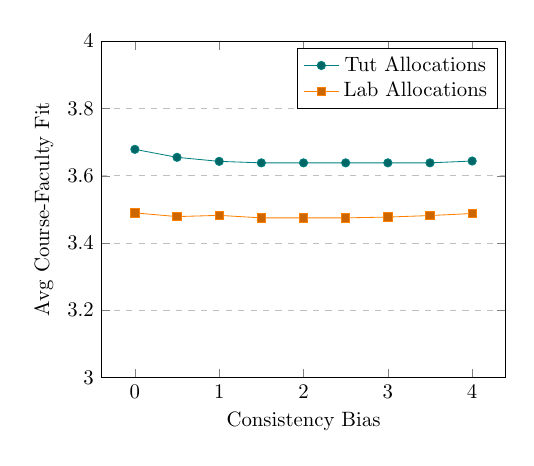
\begin{tikzpicture}[xscale=0.75, yscale=0.75]
      \begin{axis}[
          xlabel={Consistency Bias},
          ylabel={Avg Course-Faculty Fit},
          ymin=3.0, ymax=4,
          ymajorgrids=true,
          grid style=dashed,
          cycle list name=exotic,
        ]
        \addplot coordinates{
            (0, 3.678571)
            (0.5, 3.654826)
            (1, 3.642857)
            (1.5, 3.638417)
            (2, 3.638417)
            (2.5, 3.638417)
            (3, 3.638417)
            (3.5, 3.638417)
            (4, 3.643822)
          };
        \addlegendentry{Tut Allocations}
        \addplot coordinates{
            (0, 3.489613)
            (0.5, 3.478615)
            (1, 3.482281)
            (1.5, 3.474745)
            (2, 3.474745)
            (2.5, 3.474745)
            (3, 3.477189)
            (3.5, 3.481670)
            (4, 3.487780)
          };
        \addlegendentry{Lab Allocations}
      \end{axis}
    \end{tikzpicture}
    \caption{on Course-Faculty Fit}
    \label{fig:score_consistency_bias}
  \end{subfigure}
  \caption{Impact of Consistency Bias}
\end{figure}


As seen in the figure, the consistency bias has a significant impact on the number of faculty per course. As the consistency bias is increased, the number of faculty per course decreases significantly. For tutorials, 3.00 faculty per course in the absence of consistency bias, the number of faculty per course decreases to 2.38 faculty per course with a consistency bias of 1. For labs, 4.35 faculty per course in the absence of consistency bias reduces to 3.28 faculty per course with a consistency bias of 1.

An interesting observation is that the consistency bias doesn't decrease the number of faculty per course consistently for labs for a bias higher than 1. Upon further investigation, it was found that this was because faculty with a high workload limit tend to prefer to teach tutorials and labs of courses with a high number of sessions. However, because the consistency bias pushes the faculty previously allocated to lectures to also be allocated to tutorials and labs, this very high bias leads to such preferences being overridden, leading to suboptimal allocation of faculty.

It can also be seen in \autoref{fig:score_consistency_bias} that the consistency bias has a negligible impact on the course-faculty fit, thus ensuring that the consistency bias doesn't affect the quality of the allocation. The course-faculty fit of tutorials remains nearly constant at 3.65, and the course-faculty fit of labs remains nearly constant at 3.48.

This shows that the consistency bias is effective in reducing the number of faculty per course, and thus improving the consistency of courses. A consistency bias of 1 was found to be optimal for the test dataset, but this is a configurable parameter that can be adjusted based on the requirements of the institution.

\subsection{Impact of Year-wise Bias}

\begin{figure}[H]
  \begin{subfigure}[ht]{0.5\linewidth}
    \centering
    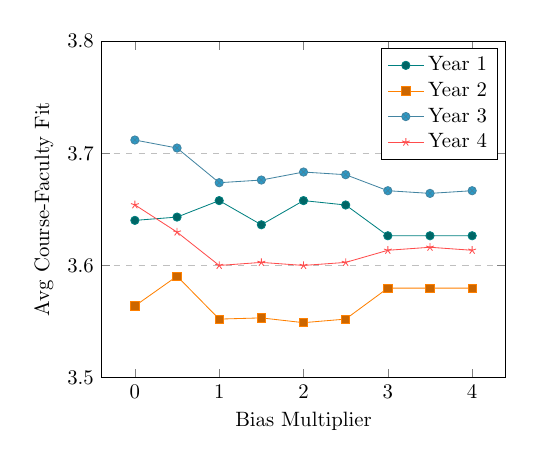
\begin{tikzpicture}[xscale=0.75, yscale=0.75]
      \begin{axis}[
          xlabel={Bias Multiplier},
          ylabel={Avg Course-Faculty Fit},
          ymin=3.5, ymax=3.8,
          ymajorgrids=true,
          grid style=dashed,
          cycle list name=exotic,
        ]

        \addplot coordinates {
            (0, 3.640196)
            (0.5, 3.643137)
            (1, 3.657843)
            (1.5, 3.636275)
            (2, 3.657843)
            (2.5, 3.653922)
            (3, 3.626471)
            (3.5, 3.626471)
            (4, 3.626471)
          };
        \addlegendentry{Year 1}
        \addplot coordinates {
            (0, 3.563830)
            (0.5, 3.590426)
            (1, 3.552128)
            (1.5, 3.553191)
            (2, 3.548936)
            (2.5, 3.552128)
            (3, 3.579787)
            (3.5, 3.579787)
            (4, 3.579787)
          };
        \addlegendentry{Year 2}
        \addplot coordinates {
            (0, 3.711905)
            (0.5, 3.704762)
            (1, 3.673810)
            (1.5, 3.676190)
            (2, 3.683333)
            (2.5, 3.680952)
            (3, 3.666667)
            (3.5, 3.664286)
            (4, 3.666667)
          };
        \addlegendentry{Year 3}
        \addplot coordinates {
            (0, 3.654054)
            (0.5, 3.629730)
            (1, 3.600000)
            (1.5, 3.602703)
            (2, 3.600000)
            (2.5, 3.602703)
            (3, 3.613514)
            (3.5, 3.616216)
            (4, 3.613514)
          };
        \addlegendentry{Year 4}

      \end{axis}
    \end{tikzpicture}
    \caption{Tutorial Allocation}
    \label{fig:tut_score_yearwise_bias}
  \end{subfigure}
  \begin{subfigure}[ht]{0.4\linewidth}
    \centering
    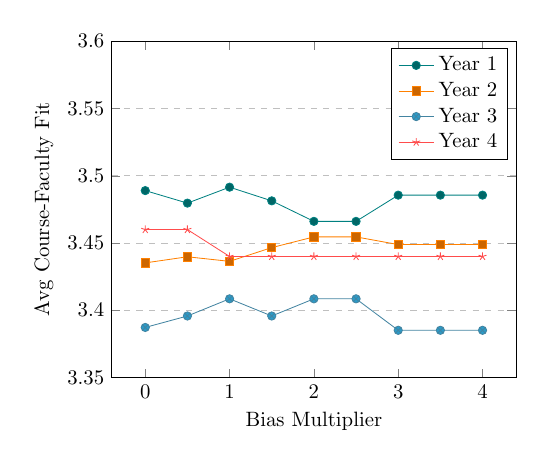
\begin{tikzpicture}[xscale=0.75, yscale=0.75]
      \begin{axis}[
          xlabel={Bias Multiplier},
          ylabel={Avg Course-Faculty Fit},
          ymin=3.35, ymax=3.6,
          ymajorgrids=true,
          grid style=dashed,
          cycle list name=exotic,
        ]
        \addplot coordinates {
            (0, 3.488983)
            (0.5, 3.479661)
            (1, 3.491525)
            (1.5, 3.481356)
            (2, 3.466102)
            (2.5, 3.466102)
            (3, 3.485593)
            (3.5, 3.485593)
            (4, 3.485593)
          };
        \addlegendentry{Year 1}

        \addplot coordinates {
            (0, 3.435227)
            (0.5, 3.439773)
            (1, 3.436364)
            (1.5, 3.446591)
            (2, 3.454545)
            (2.5, 3.454545)
            (3, 3.448864)
            (3.5, 3.448864)
            (4, 3.448864)
          };
        \addlegendentry{Year 2}

        \addplot coordinates {
            (0, 3.387234)
            (0.5, 3.395745)
            (1, 3.408511)
            (1.5, 3.395745)
            (2, 3.408511)
            (2.5, 3.408511)
            (3, 3.385106)
            (3.5, 3.385106)
            (4, 3.385106)
          };
        \addlegendentry{Year 3}

        \addplot coordinates {
            (0, 3.460000)
            (0.5, 3.460000)
            (1, 3.440000)
            (1.5, 3.440000)
            (2, 3.440000)
            (2.5, 3.440000)
            (3, 3.440000)
            (3.5, 3.440000)
            (4, 3.440000)
          };
        \addlegendentry{Year 4}
      \end{axis}
    \end{tikzpicture}
    \caption{Lab Allocation}
    \label{fig:lab_score_yearwise_bias}
  \end{subfigure}
  \caption{Impact of Year-wise Bias on Course-Faculty Fit}
\end{figure}

\autoref{fig:tut_score_yearwise_bias} and \autoref{fig:lab_score_yearwise_bias} show the impact when the default year-wise biases of 1, 0.75, 0.5, 0.25, and 0 for years 1-5 respectively are multiplied by a factor of 0 to 4. This means that for the first reading, the year-wise bias for all years is 0, and for the last reading, the biases for all years are multiplied by 4, yielding a year-wise bias of 4, 3, 2, 1, and 0 for years 1-5 respectively.

It can be seen that the year-wise bias has an impact on the course-faculty fit of tutorials, although the impact is consistent throughout. Moving from a bias multiplication factor of 0 to 1, it can be seen that the year 1 quality increases from 3.64 to 3.66 for tutorials and from 3.48 to 3.49 for labs. On the other hand, the year 4 quality decreases from 3.65 to 3.60 for tutorials and from 3.46 to 3.44 for labs. This is consistent with the expected behavior of the year-wise bias, which is to allocate earlier-year courses to the best faculty.

However, upon increasing the consistency bias further, the course-faculty fit of tutorials doesn't consistently improve. Upon further investigation, it was found that the bias had an impact on the first few iterations of the Hungarian algorithm. However, this greediness towards allocating earlier-year courses to the best faculty counteracts in the later iterations, with the earlier-year courses being allocated to worse faculty than the allocations in the absence of year-wise bias.

This can be seen in \autoref{tab:yearwise_bias_hungarian_iterations}, which shows the year 1 quality for the first 4 iterations of the Hungarian algorithm for a bias multiplication factor of 0 and 25. In theory, a bias multiplication factor of 25 should allocate all the year 1 courses to the best faculty, and thus the year 1 quality should be higher than the year 1 quality in the absence of year-wise bias. However, it can be seen that the year 1 quality is effectively lower after the first few iterations of the Hungarian algorithm. This is because the year-wise bias creates a greediness towards the best faculty for the first few iterations, but this leads to suboptimal allocations in the later iterations.

\begin{table}[H]
  \centering
  \begin{tabular}{|l|c|c|}
    \hline
    \textbf{Iteration}   & \textbf{Multiplier = 0} & \textbf{Multiplier = 25} \\ \hline
    \textbf{Iteration 1} & 3.733333                & 3.755556                 \\ \hline
    \textbf{Iteration 2} & 3.709756                & 3.724390                 \\ \hline
    \textbf{Iteration 3} & 3.703846                & 3.692453                 \\ \hline
    \textbf{Iteration 4} & 3.705263                & 3.686441                 \\ \hline
  \end{tabular}
  \caption{Year 1 Quality for the first 4 iterations of Hungarian}
  \label{tab:yearwise_bias_hungarian_iterations}
\end{table}

\subsection{Impact of Batch Size}

To check the impact of batch size, the tutorial and lab allocation algorithms were run with batch sizes of 1 to 10. The

\begin{figure}[ht]
  \begin{subfigure}[ht]{0.5\linewidth}
    \centering
    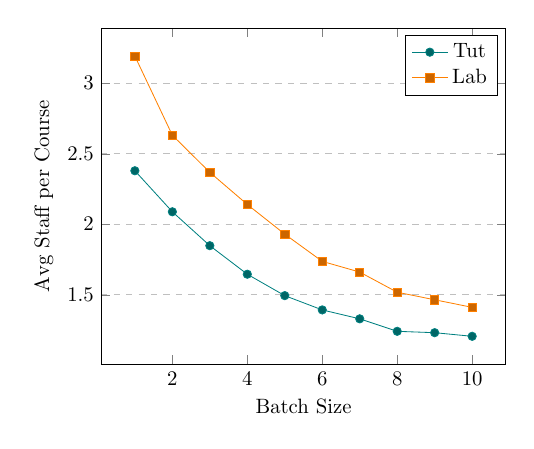
\begin{tikzpicture}[xscale=0.75, yscale=0.75]
      \begin{axis}[
          xlabel={Batch Size},
          ylabel={Avg Staff per Course},
          ymajorgrids=true,
          grid style=dashed,
          cycle list name=exotic,
        ]
        \addplot coordinates{
            (1, 2.3797468354430378)
            (2, 2.088607594936709)
            (3, 1.8481012658227849)
            (4, 1.6455696202531647)
            (5, 1.4936708860759493)
            (6, 1.3924050632911393)
            (7, 1.3291139240506329)
            (8, 1.240506329113924)
            (9, 1.2307692307692308)
            (10, 1.205128205128205)
          };
        \addlegendentry{Tut}

        \addplot coordinates{
            (1, 3.192982456140351)
            (2, 2.6315789473684212)
            (3, 2.3684210526315788)
            (4, 2.1403508771929824)
            (5, 1.9298245614035088)
            (6, 1.736842105263158)
            (7, 1.6607142857142858)
            (8, 1.5178571428571428)
            (9, 1.4642857142857142)
            (10, 1.4107142857142858)
          };
        \addlegendentry{Lab}
      \end{axis}
    \end{tikzpicture}
    \caption{on Faculty per Course}
    \label{fig:faculty_per_course_batch_size}
  \end{subfigure}
  \begin{subfigure}[ht]{0.5\linewidth}
    \centering
    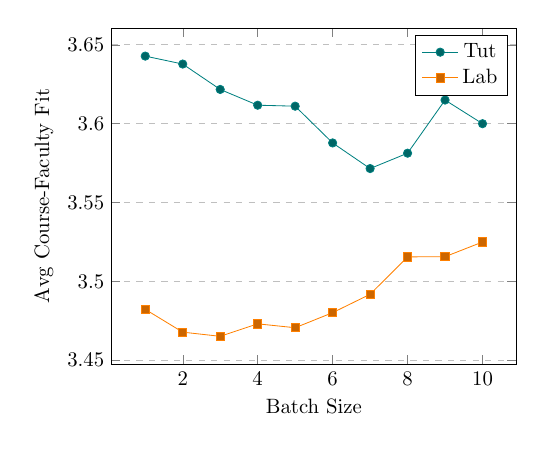
\begin{tikzpicture}[xscale=0.75, yscale=0.75]
      \begin{axis}[
          xlabel={Batch Size},
          ylabel={Avg Course-Faculty Fit},
          ymajorgrids=true,
          grid style=dashed,
          cycle list name=exotic,
        ]
        \addplot coordinates{
            (1, 3.642857)
            (2, 3.637818)
            (3, 3.621717)
            (4, 3.611728)
            (5, 3.611111)
            (6, 3.587805)
            (7, 3.571552)
            (8, 3.581308)
            (9, 3.615000)
            (10, 3.600000)
          };
        \addlegendentry{Tut}

        \addplot coordinates{
            (1, 3.482281)
            (2, 3.467829)
            (3, 3.465193)
            (4, 3.473103)
            (5, 3.470635)
            (6, 3.480189)
            (7, 3.491837)
            (8, 3.515556)
            (9, 3.515663)
            (10, 3.525000)
          };
        \addlegendentry{Lab}
      \end{axis}
    \end{tikzpicture}
    \caption{on Course-Faculty Fit}
    \label{fig:score_batch_size}
  \end{subfigure}
  \par \bigskip
  \begin{subfigure}[ht]{0.5\linewidth}
    \centering
    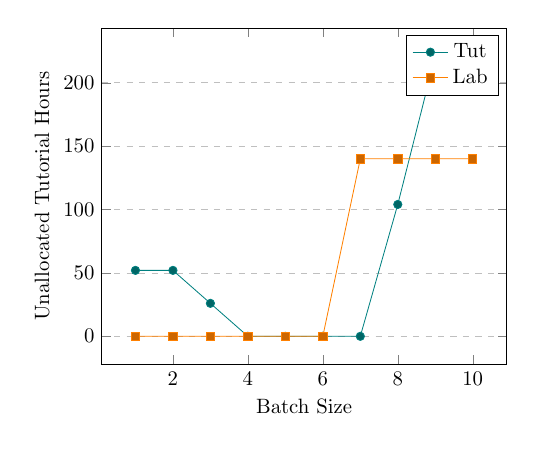
\begin{tikzpicture}[xscale=0.75, yscale=0.75]
      \begin{axis}[
          xlabel={Batch Size},
          ylabel={Unallocated Tutorial Hours},
          ymajorgrids=true,
          grid style=dashed,
          cycle list name=exotic,
        ]
        \addplot coordinates{
            (1, 52)
            (2, 52)
            (3, 26)
            (4, 0)
            (5, 0)
            (6, 0)
            (7, 0)
            (8, 104)
            (9, 221)
            (10, 221)
          };
        \addlegendentry{Tut}

        \addplot coordinates{
            (1, 0)
            (2, 0)
            (3, 0)
            (4, 0)
            (5, 0)
            (6, 0)
            (7, 140)
            (8, 140)
            (9, 140)
            (10, 140)
          };
        \addlegendentry{Lab}
      \end{axis}
    \end{tikzpicture}
    \caption{on Course-Faculty Fit}
    \label{fig:unallocated}
  \end{subfigure}
  \begin{subfigure}[ht]{0.5\linewidth}
    \centering
    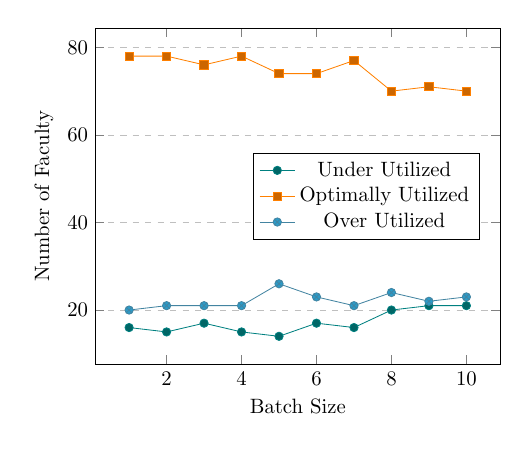
\begin{tikzpicture}[xscale=0.75, yscale=0.75]
      \begin{axis}[
          xlabel={Batch Size},
          ylabel={Number of Faculty},
          ymajorgrids=true,
          grid style=dashed,
          cycle list name=exotic,
          legend style={at={(0.95, 0.5)}, anchor=east}
        ]
        \addplot coordinates{
            (1, 16)
            (2, 15)
            (3, 17)
            (4, 15)
            (5, 14)
            (6, 17)
            (7, 16)
            (8, 20)
            (9, 21)
            (10, 21)
          };
        \addlegendentry{Under Utilized}
        \addplot coordinates{
            (1, 78)
            (2, 78)
            (3, 76)
            (4, 78)
            (5, 74)
            (6, 74)
            (7, 77)
            (8, 70)
            (9, 71)
            (10, 70)
          };
        \addlegendentry{Optimally Utilized}
        \addplot coordinates{
            (1, 20)
            (2, 21)
            (3, 21)
            (4, 21)
            (5, 26)
            (6, 23)
            (7, 21)
            (8, 24)
            (9, 22)
            (10, 23)
          };
        \addlegendentry{Over Utilized}
      \end{axis}
    \end{tikzpicture}
    \caption{on Faculty Utilization}
    \label{fig:overloading_batch_size}
  \end{subfigure}
  \caption{Impact of Batch Size}
\end{figure}

As seen in \autoref{fig:faculty_per_course_batch_size}, the batch size has a significant impact on the number of faculty per course. As the batch size is increased, the number of faculty per course decreases significantly. For tutorials, 2.38 faculty per course for a batch size of 1 decreases to 1.21 faculty per course for a batch size of 10. For labs, 3.19 faculty per course for a batch size of 1 decreases to 1.41 faculty per course for a batch size of 10. This shows that batch size has the desired effect of reducing the number of faculty per course.

\autoref{fig:score_batch_size} shows that the batch size has a mild impact on the course-faculty fit of tutorials, although the impact is consistent throughout. Moving from a batch size of 1 to 10, it can be seen that the course-faculty fit of tutorials decreases from 3.64 to 3.60. On the other hand, the course-faculty fit of labs increases from 3.48 to 3.53. This is consistent with the expected behavior of the batch size, which is to allocate earlier-year courses to the best faculty. This shows that the batch size does not necessarily have a negative impact on the course-faculty fit.

\autoref{fig:unallocated} shows that the batch size has a significant impact on the number of unallocated tutorial hours. As the batch size is increased, the number of unallocated tutorials decreases up to a certain point and then increases. For tutorials, 52 unallocated tutorial hours for a batch size of 1 decreases to 0 unallocated tutorial hours for a batch size of 4 onwards, and then shot back up after a batch size of 8 to 104 and continued increasing to 221 for a batch size of 10. For labs, 0 unallocated lab hours for a batch size of 1 increases to 140 unallocated lab hours for a batch size of 7 onwards. This shows that batch size does not have a direct correlation to the number of unallocated tutorial hours. Upon investigating the increase in the unallocated hours for tutorials for very high batch sizes, it was found that large batch sizes lead to many faculty being unable to teach certain tutorials due to the workload limits of the faculty being exceeded.

\autoref{fig:overloading_batch_size} shows that the batch size also has a significant impact on faculty utilization. Optimal utilization is defined as a 90\% to 110\% utilization, underutilization as a utilization of less than 90\%, and overutilization as a utilization of more than 110\%. As the batch size is increased, the number of optimally utilized faculty decreases slightly from 78 to 70 when moving from a batch size of 1 to 10. The number of underutilized faculty increased from 16 to 21, and the number of overutilized faculty also increased from 20 to 23 for the same batch size range. This shows that batch size has a slight negative impact on the faculty utilization, however upon looking further into the data, the change was found to be well within the acceptable limits.

With these results, it can be concluded that increased batch sizes greatly alleviate the problem of fragmentation. This outcome was significantly more impactful than the consistency bias, although a combination of both is recommended for optimal results. The optimal batch size using this approach was found to be 6, since it had the best balance of faculty per course, course-faculty fit, and faculty utilization.

\subsection{Impact of Pre-Allocation}

To check the impact of pre-allocation, the tutorial and lab allocation algorithms were run with and without pre-allocation. The dynamic adjustment of limits was intentionally disabled for this experiment since that will help highlight the unallocated tutorials and labs caused by the absence of pre-allocation. The batch size was set to 6 for this experiment.

\begin{table}[H]
  \centering
  \begin{tabular}{|l|c|c|c|c|}
    \hline
                             & \multicolumn{2}{c|}{Tutorial} & \multicolumn{2}{c|}{Lab}                                            \\ \hline
    \textbf{Metric}          & \textbf{Without Pre}          & \textbf{With Pre}        & \textbf{Without Pre} & \textbf{With Pre} \\ \hline
    Assigned Hrs             & 4862                          & 5146                     & 3637                 & 3807              \\ \hline
    Unassigned Hrs           & 1896                          & 1612                     & 1439                 & 1269              \\ \hline
    \textbf{\% Hrs Assigned} & \textbf{73.0}                 & \textbf{76.3}            & \textbf{75.0}        & \textbf{76.9}     \\ \hline
    Avg Score                & 3.60                          & 3.61                     & 3.52                 & 3.52              \\ \hline
  \end{tabular}
  \caption{Impact of Pre-Allocation}
  \label{tab:pre_allocation}
\end{table}

\autoref{tab:pre_allocation} shows the impact of pre-allocation on the tutorial and lab allocation processes. It can be seen that pre-allocation has a significant impact on the number of hours assigned, with an additional 3.3\% of tutorial hours and 1.9\% of lab hours being assigned when pre-allocation is used. This is because pre-allocation allows the algorithm to allocate tutorials and labs that have a shortage of faculty, which would otherwise be unallocated.

\subsection{Impact of Dynamic Adjustment of Limits}

As can also be seen in \autoref{tab:pre_allocation}, the absence of dynamic adjustment of limits leads to a significant number of unallocated tutorial and lab hours. This is due to a combination of uneven demand for faculty to teach certain courses, which doesn't line up with the workload limits of the faculty, and the greediness of the Hungarian algorithm which prioritizes the student feedback score for earlier iterations of the algorithm.

\begin{table}[H]
  \centering
  \resizebox{\textwidth}{!}{
    \begin{tabular}{|l|c|c|c|c|}
      \hline
                                 & \textbf{Unallocated Batches} & \textbf{Total duties limit} & \textbf{Tut limit} & \textbf{Workload limit} \\ \hline
      \textbf{Before Adjustment} & 31                           & 12                          & 6                  & 1.0                     \\ \hline
      Iteration 1                & 21                           & 12                          & 6                  & 0.1                     \\ \hline
      Iteration 2                & 15                           & 14                          & 7                  & 0.2                     \\ \hline
      Iteration 3                & 3                            & 16                          & 8                  & 0.3                     \\ \hline
      Iteration 4                & 1                            & 16                          & 8                  & 0.4                     \\ \hline
      Iteration 5                & 0                            & 18                          & 9                  & 0.5                     \\ \hline
    \end{tabular}
  }
  \caption{Impact of Dynamic Adjustment of Limits on Tutorials}
  \label{tab:dynamic_adjustment_tutorials}
\end{table}

\begin{table}[H]
  \centering
  \resizebox{\textwidth}{!}{
    \begin{tabular}{|l|c|c|c|c|}
      \hline
                                 & \textbf{Unallocated Batches} & \textbf{Total duties limit} & \textbf{Lab limit} & \textbf{Workload limit} \\ \hline
      \textbf{Before Adjustment} & 44                           & 12                          & 6                  & 1.0                     \\ \hline
      Iteration 1                & 27                           & 14                          & 7                  & 0.1                     \\ \hline
      Iteration 2                & 9                            & 16                          & 8                  & 0.2                     \\ \hline
      Iteration 3                & 6                            & 18                          & 9                  & 0.3                     \\ \hline
      Iteration 4                & 0                            & 20                          & 10                 & 0.4                     \\ \hline
    \end{tabular}
  }
  \caption{Impact of Dynamic Adjustment of Limits on Labs}
  \label{tab:dynamic_adjustment_labs}
\end{table}

\section{Summary}

This chapter presented the approach towards tutorial allocation and lab allocation. This approach involved the use of the Hungarian algorithm to allocate tutorials and labs to faculty. The approach also involved the use of a consistency bias in the cost matrix, and the use of batching to reduce fragmentation. The cost matrix was also modified to include the year-wise bias, which allocates earlier-year courses to the best faculty, and teaching duty limits to ensure that faculty are not overworked.

As part of the allocation process, the tutorials were first pre-allocated to ensure that tutorials with a shortage of faculty were allocated. Then it used the above approach to allocate the tutorials. Finally, if any tutorials were left unallocated, the workload limits and teaching duty limits of the faculty were dynamically adjusted to ensure that the unallocated tutorials were allocated.

The approach was then tested on the test dataset. The results showed that the approach was able to allocate tutorials and labs with a high course-faculty fit, and a low number of faculty per course, while maintaining a high faculty utilization. It was shown that the consistency bias was able to reduce the number of faculty per course, and the batching was very effective in reducing fragmentation as well. The year-wise bias was shown to not be very effective in allocating the earlier-year courses to the best faculty. The dynamic adjustment of limits was shown to be very effective in reducing the number of unallocated tutorials and labs without significantly overworking the faculty.
